\section{Methoden zur Positionsbestimmung}
\label{sec:methoden}

\begin{frame}
\frametitle{Methoden zur Positionsbestimmung}

\begin{itemize}
   \item Anchor/Beacon Nodes
   \item Signalstärkemessung
   \item Hop Count
   \item Zeitmessung
   \item Auftreffwinkel
\end{itemize}

\end{frame}

\begin{frame}
\frametitle{Anchor/Beacon Nodes}

\begin{itemize}
  \item Die Anchor Nodes haben eine bekannte Position (z.B. GPS oder fest einprogrammiert)
  \item Für ein globales 2D Koordinatensystem sind 3 nicht linear angeordnete Anchor Nodes erforderlich, für ein 3D KS entsprechend 4.
  \item Es wird nun entweder ein relatives Koordinatensystem mit allen nicht Anchor Nodes erstellt und dann mit Hilfe dieser in ein globales überführt oder es wird mit Hilfe der Anchor Nodes direkt jede einzelne Postion der Nodes bestimmt
\end{itemize}
\end{frame}

\begin{frame}
\frametitle{Anchor/Beacon Nodes - Vorteile/Nachteile}

\begin{itemize}
  \item Vorteile
  \begin{itemize}
    \item Für globales KS unerlässlich
    \item Vereinfachung der Positionsberechnung der anderen Nodes
  \end{itemize}
  \item Nachteile
  \begin{itemize}
    \item GPS für Anchor Nodes sehr teuer und verbrauchen viel Energie
    \item Vorprogrammieren von festen Positionen bei großen Sensornetzen sehr aufwendig und nur bei festen Sensornetzen überhaupt möglich
  \end{itemize}
\end{itemize}
\end{frame}

\begin{frame}
\frametitle{Signalstärkemessung}

\begin{itemize}
  \item mmmm
\end{itemize}
\end{frame}

\begin{frame}
\frametitle{Hop Count}

\begin{itemize}
  \item mmmm
\end{itemize}
\end{frame}

\begin{frame}
  \frametitle{Hop Count}

  \begin{center}
  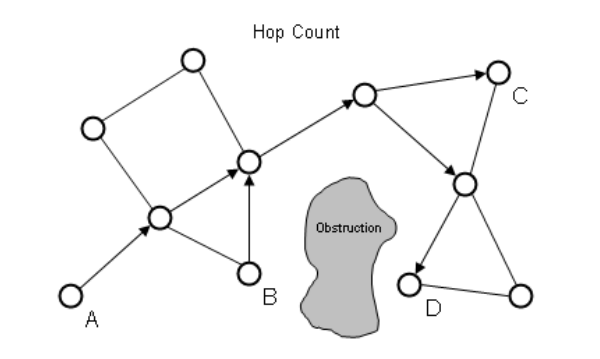
\includegraphics[scale=0.5]{img/hop_count1}
  \\~\\
  Messung A $\to$ C = 4 Hops - Messung B $\to$ D = 4 Hops
  \end{center}
\end{frame}

\begin{frame}
\frametitle{Zeitmessung}

\begin{itemize}
  \item mmmm
\end{itemize}
\end{frame}

\begin{frame}
\frametitle{Auftreffwinkel}

\begin{itemize}
  \item mmmm
\end{itemize}
\end{frame}
